% !TEX root = ../thesis.tex
\chapter{Architecture}\label{cha:architecture}
Designing and building a general purpose \gls{CPU} includes a lot of architectural decisions which will decide how well the \gls{CPU} performs, how complex it is and so on.
The goal for the \gls{EDiC} was to build a \gls{CPU} that is capable of interacting with extensible \gls{IO} device such as the VT-100 but at the same time simple enough to easily understand its workings, such that it is suited to be used in education.

\section{Design Decisions}
First of all, there are several decisions about the general structure of a \gls{CPU} that need to be made.
These decisions greatly influence how the \gls{EDiC} can be structured into modules and how the final hardware build is setup.
Another important factor towards architectural structure is the fact that the final hardware build of the \gls{CPU} is be based on the 74-series of \gls{TTL} \glspl{IC}.

\subsection{8 bit bus width}
Most current era \glspl{CPU} employ a 32 bit or 64 bit bus to handle large numbers and large amounts of data.
This, however, is not feasible when using 74-series \glspl{IC} and at the same time targeting an easy to understand hardware build.
Some early \glspl{CPU} build with similar \glspl{IC} worked with only 4 bits.
This can work very well for specific applications but for the most arithmetics and data handling 8 bits are more practical.
The \gls{EDiC} will, therefore, use an 8 bit bus for data with a integer range of -128 to 127 or 0 to 255 for unsigned integers.

One of the major limitation of an overall 8 bit bus is the addressable memory space.
With only 8 bit for the memory address, the maximum amount of memory addressable is 256 bytes.
In a first prototype of the \gls{CPU} the memory space was tripled by providing 256 bytes of instruction memory besides 256 bytes of \gls{ROM} for instruction immediate values and 256 bytes of addressable \gls{SRAM}.
However, especially with a \gls{CISC} architecture (see \cref{sec:cisc}), the limited \gls{SRAM} memory space greatly limits the overall complexity of programs that can be executed.
Additionally, more complex programs or even small operating systems are impossible to fit into 256 instructions.

Therefore, it was decided to extend the \gls{PC} and the memory addresses to 16 bit, which yields 65536 bytes of addressable \gls{SRAM} and theoretically 65536 instructions\footnote{The largest feasible \gls{EEPROM} available used for instruction memory has only 15 address bits and with that only 32768 8 bit words of data.}.
However, this raises problems of where the 16 bit addresses come from when all the registers and the memory only store 8 bit.
The solution for the \gls{EDiC} is presented in \cref{sec:addrLogic} when explaining the different modules of the \gls{EDiC}.

\subsection{Datapath Architecture - Multicycle CISC}\label{sec:cisc}
In most \glspl{CPU} an instruction is not done in one clock cycle but it is divided into several steps that are done in sequence.
There are two general approaches that are called \emph{Multicycle} and \emph{Pipelining} \cite{PattersonDavid2016RuRD}.
Multicycle means that all the steps of one instruction are performed sequentially and a new instruction is only dispatched after the previous instruction is finished.
This is usually used when implementing \glspl{CISC}, where one instruction can be very capable \cite{chen_novick_shimano_2000}.
For example an add instruction in \gls{CISC} could fetch operands from memory, execute the add and write the result back to memory.
\glspl{RISC} on the other hand would need three independent instruction to load operands from memory into registers, do the addition and write the result back to memory.

In Pipelining there are fixed steps each instruction goes through in a defined order and the intermediate results are stored in so called pipeline registers.
Each pipeline step is constructed in such a way that it does not intervene with the others.
Therefore, it is, in theory, possible to dispatch a new instruction each cycle even though the previous instruction is not yet finished.
A typically 5-step pipeline would consist of the following steps \cite{PattersonDavid2016RuRD}:
\begin{enumerate}
  \item \textbf{Instruction Fetch}: The instruction is retrieved from memory and stored in a register.
  \item \textbf{Instruction Decode}: The fetched instruction is decoded into control signals (and instruction specific data) for all the components of the \gls{CPU}.
  \item \textbf{Execute}: If arithmetic or logical operations are part of the instruction, they are performed.
  \item \textbf{Memory Access}: Results are written to the memory and/or data is read from memory.
  \item \textbf{Writeback}: The results are written back to the registers.
\end{enumerate}
However good the performance of a pipelined \gls{CPU} is, it also comes with challenges.
Those include a greater resource usage because all intermediate results need to be stored in pipeline registers.
Additionally, branch instructions\footnote{Branch Instructions change the \gls{PC} and with that the location from which the next instruction is to be fetched. This is required for conditional and looped execution.} pose a greater challenge because at the moment, the \gls{CPU} execute the branch the following instructions have already been dispatched.
This means that the pipeline needs to be flushed (i.e. cleared), performance is lost and more logic is required.
It also noteworthy that branch prediction and pipeline flushes can be quite vulnerable as recently shown in CVE-2017-5753 with the Spectre bug \cite{CVE-2017-5753}.

Therefore, the \gls{EDiC} is to built as a Multicycle \gls{CISC}.

\subsection{Single-Bus Oriented}
The decision for a Multicycle \gls{CPU} also enabled the architecture to be single-bus oriented.
This means that all modules (e.g. the \gls{ALU} or the memory) are connected to a central bus for data transfer.
The central bus is then used as a multi-directional data communication.
To allow this in hardware, all components that drive the bus (i.e. ``send'' data) need to have a tri-state driver.
A tri-state driver can either drive the bus with a defined `0' (low voltage) or `1' (high voltage) or not drive the bus (high impedance) which allows other tri-state drivers on the same bus to drive it.
That way an instruction which fetches a word from the memory from an address stored in a register, adds a register value to it and stores it in a register could consist of the following steps:
\begin{enumerate}
  \item Instruction Fetch
  \item Instruction Decode
  \item Memory Address from register over \emph{bus} to memory module
  \item Memory Access
  \item Data from memory module over \emph{bus} to \gls{ALU} input
  \item \gls{ALU} operation
  \item Data from \gls{ALU} output over \emph{bus} to register
\end{enumerate}
With such an architecture it is possible to avoid large multiplexers and keep the overall architecture simple.


\section{Modules}
The design has been split into 7 rather independent modules of varying complexity which mainly interface with each other over the bus and control signals.
\subsection{\glsxtrfull{ALU}}\label{sec:alu}
\begin{figure}[t]
  \centering
  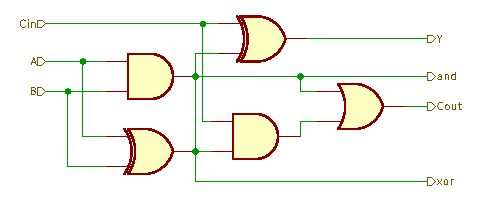
\includegraphics[width=\textwidth]{full_adder.pdf}
  \caption{1 bit full adder with the usual A, B and Carry inputs and Y and Carry outputs as well as the XOR and AND outputs.}
  \label{fig:full_adder}
\end{figure}
An \gls{ALU} is the computational core of any \gls{CPU} as it performs all the calculations.
The \gls{ALU} of the \gls{EDiC} is by design simple with only 4 different operations plus an option to invert the second input.
The result of the \gls{ALU} is stored in a result register which can drive the bus to store the result in a register or memory.
For simplicity, the first input of the \gls{ALU} ($A$ input) is directly connected to the register file (\cref{sec:regs}) and only the second input ($B$ input) is accessible from the bus.
This limits the possibilities of instructions, however, if both inputs should have been driven by the bus, every \gls{ALU} instruction would have taken three instead of two cycle limited by the bus (first cycle $A$ input, second cycle $B$ input, third cycle result).

The \gls{ALU} consists of an 8 bit ripple carry full adder and a barrel shifter.
The operations are controlled by three control signals: The first two bits select which \gls{ALU} operation to perform and the third bit modifies the operation to perform.
The possible operations are shown in \cref{tab:aluOp}.
For the adder, the third bit inverts the $B$ input when active (All input bits are XORed with the control bit) and is used as the carry in of the adder.
This negates the $B$ input in twos complement and, therefore, subtracts it from the $A$ input.
For the barrel shifter, the third bit reverses the shift direction.

\begin{table}
  \centering
  \renewcommand{\arraystretch}{1.25}
  \caption{Summary of the available \gls{ALU} operations.}
  \label{tab:aluOp}
  \begin{tabularx}{.8\textwidth}{ |c|c|c||X| }
    \hline
    aluOp[1] & aluOp[0] & aluSub & Resulting Operation             \\\hline\hline
    0        & 0        & 0      & ($A + B$) Addition              \\\hline
    0        & 0        & 1      & ($A - B$) Subtraction           \\\hline
    0        & 1        & 0      & ($A \land B$) AND               \\\hline
    0        & 1        & 1      & ($A \land \overline{B}$)        \\\hline
    1        & 0        & 0      & ($A \veebar B$) XOR             \\\hline
    1        & 0        & 1      & ($\overline{A \veebar B}$) XNOR \\\hline
    1        & 1        & 0      & ($A \gg B$) logical shift right \\\hline
    1        & 1        & 1      & ($A \ll B$) logical shift left  \\\hline
  \end{tabularx}
\end{table}
The XOR and AND operations shown in \cref{tab:aluOp} are chosen because they are already implemented in the half-adders and no additional logic is required to implement them.
A complete 1 bit full-adder of the \gls{EDiC} is shown in \cref{fig:full_adder}.

\begin{sidewaysfigure}[p]
  \centering
  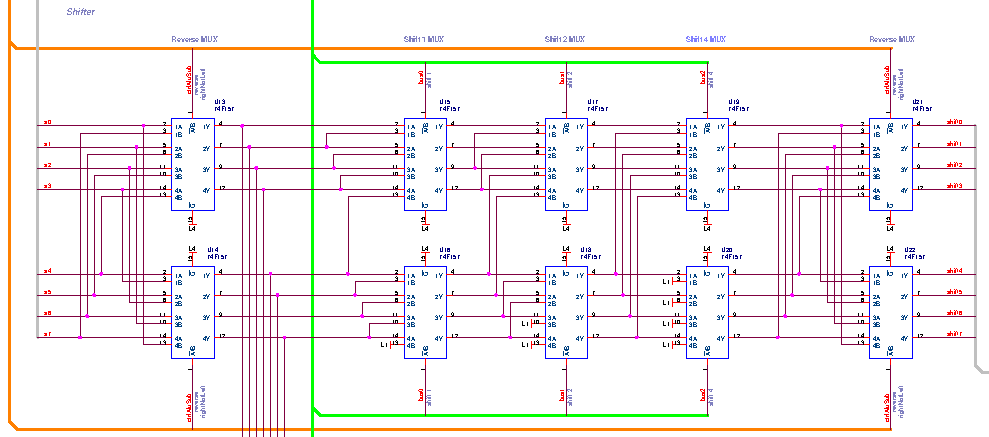
\includegraphics[width=\linewidth]{barrel_shifter.pdf}
  \caption{8 bit bidirectional barrel shifter.}
  \label{fig:barrel_shifter}
\end{sidewaysfigure}
It was desirable to include a barrel shifter to have the possibility to improve multiply operation with a shift and add approach instead of repeated addition.
The barrel shifter works by 3 consecutive multiplexers shifting by 1, 2 or 4 bit to the right that are controlled by the first 3 bit of the (not inverted) $B$ input.
To also allow shifting to the left there is one multiplexer before the three shift multiplexers to invert the order of bits and another one after the shifting to reorder the bits.
In \cref{fig:barrel_shifter} a bidirectional barrel shifter implemented with the \texttt{74F157} is visualized. The \texttt{74F157} implements four 2 to 1 multiplexer and, therefore, 2 chips are needed for a full 8 bit 2 to 1 multiplexer.

The \gls{ALU} also provides four flags which are used for condition execution.
The Zero (all result bits are zero) and Negative (The \gls{MSB} of the result) flag are both very easy to derive and were the only ones included in the prototype.
However, the experience of programming for the \gls{CPU} showed that it is desireable to be able to work with more advanced \gls{ALU} flags when programming more complex functions.
Having only Zero and Negative Flags, for example, does not allow unsigned operations of the full width\footnote{An overflow detection is not possible and with that a greater or less than comparison cannot be done.} which is especially important with only 8 data bits.
It limits unsigned operations to only 0-127 even though the \gls{ALU} would be capable of calculations with 0-255.

A lot of modern \glspl{CPU} feature many different flags with the Intel 64\textsuperscript{\textregistered} and IA-32 \gls{CPU} having about 20 different flags \cite[Section~3.4.3]{intelx86}.
However, the popular ARM Architecture has a rather unique but very capable system for conditional execution which relies on only the four most used \gls{ALU} flags.
The \gls{EDiC} uses the same flags and their functions are as follows:
\begin{itemize}
  \item \textbf{N} The \emph{Negative} flag indicates that the result is negative and is set if the 8th bit of the \gls{ALU} result (\gls{MSB}) is \texttt{'1'}.
  \item \textbf{Z} The \emph{Zero} flag indicates that the result is 0 and is set if all 8 result bits are 0.
  \item \textbf{V} The \emph{Overflow} flag indicates that an overflow occurred and is set if the carry in and carry out of the 8th full-adder are different.
  This detects arithmetic overflows for signed two's-complement calculations.
  \item \textbf{C} The \emph{Carry} flag is the carry out bit of the adder for adding and subtracting.
  For logical operations (\texttt{XOR} and \texttt{AND}) the carry flag has no meaning and for shifting operations it equals the last bit that was ``carried out'' (or is unchanged if shifting by 0 bits).
\end{itemize}
\subsection{Register File}\label{sec:regs}
As is typical with \glspl{CISC} the \gls{CPU} does not need many general purpose registers and the register file can be kept simple with only two registers.
The register file has one write port (from the bus) and two read ports of which one reads to the bus and the other is directly connected to the $A$ input of the \gls{ALU}.
All ports can access both registers.
\subsection{\glsxtrfull{PC} \& Instruction Register}
The \gls{PC} is a special 16 bit register which is used to store the address for the current instruction.
Usually it is incremented by one for each instruction.
However, it is also possible to load the \gls{PC} from an instruction immediate (see below) or from the memory (\cref{sec:memory}).
The first option is used for branch instruction while the second option is used for returning from a function, which is explained in more detail in \cref{sec:stack}.
The value of the \gls{PC} is used as address for the instruction \glspl{EEPROM} and can also be driven to the memory for storing the return address for function calls.

Each instruction of the \gls{EDiC} is stored in a 24 bit register of which 8 bits are the instruction and 16 bits represent an optional instruction immediate.
It can be used as an address for the memory/\gls{PC} (16 bit) or as data (8 bit) driven to the bus.
The instruction is directly forwarded to the control logic (\cref{sec:control}).

\subsection{Control Logic}\label{sec:control}
The control logic's job is to decode the current instruction and provide all the control signals for each cycle for any instruction.
What kind of control signals exist in the \gls{EDiC} is explained after all the modules are described in \cref{sec:controlSignals}.
For keeping track which cycle of each instruction is currently executing, a 3 bit synchronous counter is used.
Each control signal could be derived by a logical circuitry with 13 inputs: 8 bits instruction, 4 bits \gls{ALU} flags and 3 bits cycle counter.
However, designing these logic circuits is a lot of work, takes up a lot of space and cannot be changed easily later on.
Therefore, an \gls{EEPROM} is used where the 13 bits that define one cycle of one specific instruction are used as addresses.
The control signals then are the data bits of the word that is stored at the specific address in the \gls{EEPROM}.
How the \gls{EEPROM} is programmed with the correct data is explained in depth in \cref{sec:microcode}.

One special case are the 3 bits \gls{ALU} opcodes.
They are not decoded the usual way from the instruction but are directly take from the 3 \glspl{LSB} of the instruction.
This is done to reduce the storage requirements for the decoding \glspl{EEPROM}.
For instructions that use the \gls{ALU}, the 3 \glspl{LSB} need to be set accordingly but for all other instructions, the three bits can be used as usual for decoding the instruction because it does not matter what the combinatorial part of \gls{ALU} does.

The first two cycles of each instruction need to be taken in special consideration because the instruction register is not yet loaded with the next instruction, because it is still being fetched and decoded.
However, the instruction fetch and decode are always the same for each instruction, which means that all memory locations where the cycle counter is equal to 0 or 1 are filled with the control signals for an instruction fetch and decode.

\subsection{Memory}\label{sec:memory}
The memory module became the most complex module because it includes not only the main memory of the \gls{CPU} in form of an asynchronous \gls{SRAM} but also includes a lot of addressing logic for the 16 bit addresses.

The addressing logic is required because the \gls{EDiC} has 16 bit addresses with only an 8 bits data bus.
However, the \gls{EDiC} also features memory mapped \gls{IO} and a stack implementation which further complicate the addressing logic.
Both these features and the addressing logic is described below.

\subsubsection{Memory Mapped \gls{IO}}
Input and Output is one of the most important factors of any \gls{CPU} besides the computing capabilities which are mostly defined by the \gls{ALU}.
The first prototype showed that using individual instructions for \gls{IO} which directly read from and write to the bus are limiting the usability quite a lot.
A common way to extend the \gls{IO} capabilities is to use so called memory mapped \gls{IO}.
This works by splitting the address space between actual memory and \gls{IO} devices.
Then every \gls{IO} operation is performed as a usual memory access but the memory chip does not receive the access and the \gls{IO} device addressed performs the operation.
In the \gls{EDiC} the memory address is decoded in such a way, that accesses to addresses \texttt{0xfe00} to \texttt{0xfeff} are performed by any connected \gls{IO} devices.
For this to work, the lower 8 address bits, the bus and memory control signals - i.e. write enable, read enable and \gls{IO} chip enable (active when the upper 8 address bits are \texttt{0xff}) - are exposed for \gls{IO} devices to connect to.

\subsubsection{Stack Implementation}\label{sec:stack}
A feature that has been thoroughly missing from the prototype \gls{CPU} is a kind of stack implementation.
The stack is essential to the workings of the very important programming paradigm \emph{functions}.
When calling functions, the return address is usually (automatically) stored on the stack where also function local variables can be stored.
This allows functions to be called recursively and also simplifies the written program code compared to simple branching.

However, a typical stack implementation as in modern \gls{CPU} architectures like ARM is rather complex.
It requires a \gls{SP} register which usually is accessible like any other general purpose register and can be directly used as an address.
This includes using it as operand for arithmetic operations which is not possible when the bus width is only 8 bits but the \gls{SP} needs to be 16 bits wide to be used as an address.
Therefore, the \gls{EDiC} uses an unique approach to the stack:

Similarly to the memory mapped \gls{IO} it was decided to implement the \gls{SP} as an 8 bit register which can be incremented and decremented at function calls and returns, respectively.
Every time a memory access is performed where the upper 8 bits of the address equal \texttt{0xff}, a 17th address bit is set and the upper 8 address bits are replaced by the current value of the \gls{SP}.
For example: The \gls{SP}  is currently \texttt{0x21} and a memory access to the address \texttt{0xff42} is performed.
Then the actual address at the memory \gls{IC} is \texttt{0x1\_2142}.

This allows each function (which has a unique \gls{SP} value on the current call stack) to have 256 bytes of function local memory.
In the \emph{call} instruction, the \gls{EDiC} automatically stores the return address (next \gls{PC} value) at address \texttt{0xffff}, which is \texttt{0x1\_\{sp\}ff} after translation.
To store the whole 16 bit return address, a second memory \gls{IC} is used in parallel which only needs 256 bytes of storage.
In the hardware build of the \gls{EDiC} the same \gls{SRAM} \gls{IC} as for the main memory is used because it is cheaply available and the built is simplified by not using more different components.
The call and return instructions are further described in \cref{sec:instructionSet}.

Usually, the stack is also used to store parameters for a function call.
In the \gls{EDiC}, this can be achieved by providing a special \emph{store} and \emph{load} instruction which access the stack memory with an increment \gls{SP}.
This way it is possible to store parameter before calling a function and it is also possible to retrieve modified values after the call\footnote{This is important when a function takes memory pointers as parameters and modifies the memory content. For example a string parsing function could take a pointer to the start of the string, parse some characters as a number, return its number representation and modify the parameter such that it points to where the parsing stopped.}.
The calling convention for the \gls{EDiC} is further described in \cref{sec:callingConvention}.

\subsubsection{Addressing Logic}\label{sec:addrLogic}
With increasing the address width to 16 bit and also adding more functionality to the memory access, the addressing logic has become more complex.
There are two main sources for memory addresses: The new 16 bit \gls{MAR} which can be written to from the bus and secondly the 16 bit instruction immediate.
As the bus is only 8 bits wide, there is a special instruction to write to the upper 8 bits of the \gls{MAR} and the lower bits are written in the memory access instruction.
This can be used when a memory address is stored in registers and is needed when looping through values in the memory like arrays.
When accessing addresses known at compile time, the 16 bit instruction immediate can be directly used as an address, preserving the \gls{MAR}.
These two sources of addresses are then decoded to either select the stack (upper 8 bits equal \texttt{0xff}), memory mapped \gls{IO} (\texttt{0xfe}) or regular memory access.
The chip enable of the main memory is only asserted when performing stack and regular memory accesses while the \gls{IO} chip enable is only asserted when the upper 8 bits are \texttt{0xfe}.
Additionally, the 17th address bit is asserted when stack access is performed and the upper 8 bits of the address are replaced with the \gls{SP} in this case.

\subsection{Input \& Output}\label{sec:IO}
The \gls{EDiC} can interface with different \gls{IO} devices connected to it via the memory mapped \gls{IO}.
For evaluation and debugging, the \gls{EDiC} includes one \gls{IO} device at address \texttt{0x00} which can be read from and written to.
The value to be read can be selected by the user with two hexadecimal 8 bit switch and the values written to the address \texttt{0x00} are displayed with a 2 digit display.
This allows simple programs to run independently of external \gls{IO} devices.

\subsection{Clock, Reset \& Debugging}\label{sec:clock}
An important feature when developing a \gls{CPU} is debugging capabilities.
The initial prototype could at least step the clock cycle by cycle.
However, as programs get more complex this feature quickly becomes less useful as each instruction is made of several cycles and when a problem occurs after several hundred instructions it is infeasible to step through all cycles.
Additionally, the usual application developer does not want to step through each cycle but rather step through each instruction, assuming that the instruction set works as intended.
Another important debugging feature is the use of breakpoints where the \gls{CPU} halts execution when the \gls{PC} reaches a specific address.

In the \gls{EDiC} halting was not realized by stopping the clock completely but rather by inhibiting the instruction step counter increment.
This has the advantage that the clock is not abruptly pulled to 0 or 1 and, therefore, no spikes on the clock line can occur.
To implement a cycle by cycle stepping mode, the halt signal is de-asserted for only one clock cycle, which in turn increments the step counter only once.
To step whole instructions, the halt signal is de-asserted until the instruction is finished (marked by a control signal that is asserted at the end of each instruction from the control logic).
In breakpoint mode, the halt signal is controlled from a comparator that compares the \gls{PC} and a 16 bit user input, asserting the halt signal when those two equal.
As soon as the \gls{CPU} halts, the user can then switch to stepping mode and debug the specific instruction of the program.
As soon as the \gls{CPU} halts, the user can then switch to stepping mode and debug the specific instruction of the program.
The user can freely switch between these modes with switches and buttons provided on the lower side of the \gls{PCB} in \cref{fig:EDiCSnake}.

\section{Control Signals}\label{sec:controlSignals}
The \gls{EDiC} has 24 control signals which define what the current cycle does:
\begin{itemize}
  \item \texttt{aluYNWE} - \gls{ALU} output register write enable (active low): Connects to the clock enable input of the \gls{ALU} output register.
  \item \texttt{aluNOE} - \gls{ALU} output enable (active low): Enables the Three State buffer to drive the bus with the value of the \gls{ALU} output register.
  \item \texttt{reg0NWE} - Register 0 write enable (active low): Connects to the clock enable input of the register 0.
  \item \texttt{reg1NWE} - Register 1 write enable (active low): Connects to the clock enable input of the register 1.
  \item \texttt{regAluSel} - Register Select for the \gls{ALU} A input: When 0, sets register 0 as A input to the \gls{ALU}, otherwise, register 1.
  \item \texttt{reg0BusNOE} - Register 0 bus output enable (active low): Drives the bus with the value of register 0.
  \item \texttt{reg1BusNOE} - Register 1 bus output enable (active low): Drives the bus with the value of register 1.
  \item \texttt{memPCFromImm} - load data for \gls{PC} from instruction immediate: Selects the load input of the \gls{PC} to be from the instruction immediate instead of from the memory.
  \item \texttt{memPCNEn} - \gls{PC} enable (active low): enables the \gls{PC} to load data or increment by one depending on the next control signal.
  \item \texttt{memPCLoadN} - \gls{PC} load and not increment (active low): When 0 load the \gls{PC} with the data specified by \texttt{memPCFromImm}, otherwise, increment the \gls{PC} by one.
  \item \texttt{memPCToRamN} - \gls{PC} output enable (active low): Drives the bus and ram2data with the value of the \gls{PC}.
  \item \texttt{memSPNEn} - \gls{SP} enable (active low): enable the \gls{SP} to be incremented or decremented depending on the next control signal.
  \item \texttt{memSPUp} - \gls{SP} increment not decrement: When 1, increment the \gls{SP}, otherwise, decrement.
  \item \texttt{memInstrNWE} - Instruction write enable (active low): Connects to the clock enable input of the instruction register.
  \item \texttt{memInstrNOE} - Instruction output enable (active low): Drives the bus with the lower 8 bits of the instruction immediate.
  \item \texttt{memMar0NWE} - \gls{MAR} bits 7..0 write enable (active low): Connects to the clock enable input of the lower 8 bits of the \gls{MAR}.
  \item \texttt{memMar1NWE} - \gls{MAR} bits 15..8 write enable (active low): Connects to the clock enable input of the upper 8 bits of the \gls{MAR}.
  \item \texttt{memInstrImmToRamAddr} - \gls{RAM} address from instruction immediate and not \gls{MAR}: When 1, use the instruction immediate as address for the memory, otherwise, use the \gls{MAR} content.
  \item \texttt{memRamNWE} - Memory write enable (active low): Connects to the write enable input of the \gls{SRAM} and \gls{IO}.
  \item \texttt{memRamNOE} - Memory output enable (active low): Drives the bus with the value of the \gls{SRAM} or \gls{IO} depending on the memory address (\cref{sec:memory}).
  \item \texttt{instrFinishedN} - Instruction finished (active low): Is asserted at the last active cycle of the instruction to reset the step counter to 0\footnote{the instruction finished signal is also used for the debugger to detect the end of an instruction and halt when stepping through instructions and not single cycles.}.
  \item \texttt{busFFNOE}\footnote{Was added in the component verification and is explained in \cref{sec:eval_bus}.} - Drive \texttt{0xff} to the bus (active low): Connects to the output enable input of the constant \texttt{0xff} driver.
\end{itemize}

\section{Final Instruction Set}\label{sec:instructionSet}
This section describes all available instructions, what they do and which instruction cycle performs which steps of the instruction.
Each instruction starts with the same two cycles for instruction fetching.
The parameters of each instruction and how the instructions are programmed is shown in \cref{sec:asm_instr}.
\subsection{\glsxtrshort{ALU} operations}
The \gls{EDiC} supports a wide variety of instructions that perform \gls{ALU} operations.
All these operations take two arguments which are used for one of the possible operations shown in \cref{tab:aluOp}.
Each \gls{ALU} operation modifies the status flags.
\begin{itemize}
  \item \emph{Register x Register:} Takes two registers as parameter and the result is stored in the first parameter.

  Cycles:
  \begin{enumerate}
    \item Both register to \gls{ALU} A and B input, write enable of \gls{ALU} result register.
    \item Write content of \gls{ALU} result register into first parameter register.
  \end{enumerate}

  \item \emph{Register x Register (no write back):} Takes two registers as parameter and the result is only calculated for the status flags.

  Cycles:
  \begin{enumerate}
    \item Both register to \gls{ALU} A and B input, write enable of \gls{ALU} result register.
  \end{enumerate}

  \item \emph{Register x Memory (from Register):} Takes one register as \gls{ALU} A input and a second register which is used as a memory address for the \gls{ALU} B input.
  The result is stored in the first register.

  Cycles:
  \begin{enumerate}
    \item Second register is stored in the lower 8 bits of the \gls{MAR}\footnote{The upper 8 bits of the \gls{MAR} should be set beforehand}.
    \item Address decoding.
    \item First register and memory content as A and B inputs, write enable of the result register.
    \item Write content of \gls{ALU} result register into first parameter register.
  \end{enumerate}

  \item \emph{Register x Memory (from immediate):} Takes one register as \gls{ALU} A input and a 16 bit value as immediate which is used as a memory address for the \gls{ALU} B input.
  The result is stored in the first register.

  Cycles:
  \begin{enumerate}
    \item Address decoding.
    \item First register and memory content as A and B inputs, write enable of the result register.
    \item Write content of \gls{ALU} result register into first parameter register.
  \end{enumerate}

  \item \emph{Register x Memory (from immediate, no write back):} Takes one register as \gls{ALU} A input and a 16 bit value as immediate which is used as a memory address for the \gls{ALU} B input.
  The result is only calculated for the status flags.

  Cycles:
  \begin{enumerate}
    \item Address decoding.
    \item First register and memory content as A and B inputs, write enable of the result register.
  \end{enumerate}

  \item \emph{Register x Immediate:} Takes one register as \gls{ALU} A input and an 8 bit value as immediate  for the \gls{ALU} B input.
  The result is stored in the first register.

  Cycles:
  \begin{enumerate}
    \item Register and immediate value as A and B inputs and write enable of the result register.
    \item Write content of \gls{ALU} result register into first parameter register.
  \end{enumerate}

  \item \emph{Register x Immediate (no write back):} Takes one register as \gls{ALU} A input and an 8 bit value as immediate  for the \gls{ALU} B input.
  The result is only calculated for the status flags.

  Cycles:
  \begin{enumerate}
    \item Register and immediate value as A and B inputs and write enable of the result register.
  \end{enumerate}
\end{itemize}

\subsection{Memory operations} Some \gls{ALU} operations also include reading values from memory.
However, the \gls{EDiC} features a lot more memory operations which are detailed below.
As all memory operations may perform memory mapped \gls{IO} operations, special care must be taken to allow asynchronous \gls{IO} devices to function as well.
This means that for each memory access, the address setup and hold must be an individual cycle, resulting in a 3 cycle memory access.
\begin{itemize}
  \item \emph{Load from register address:} Takes the second register parameter as the lower 8 bits of the memory address and writes the memory content to the first register.

  Cycles:
  \begin{enumerate}
    \item Second register to lower \gls{MAR}.
    \item Memory address setup.
    \item Memory read access and write back to first register.
    \item Memory address hold.
  \end{enumerate}

  \item \emph{Load from immediate address:} Takes a 16 bit immediate as the memory address and writes the memory content to the register.

  Cycles:
  \begin{enumerate}
    \item Memory address setup.
    \item Memory read access and write back to first register.
    \item Memory address hold.
  \end{enumerate}

  \item \emph{Load from immediate address with incremented \gls{SP}:} Takes a 16 bit immediate as the memory address and writes the memory content to the register.
  However, before the memory access, the \gls{SP} is incremented and after the access, the \gls{SP} is decremented again.
  This is used to access parameters for subfunctions.

  Cycles:
  \begin{enumerate}
    \item Increment Stack Pointer.
    \item Memory address setup.
    \item Memory read access and write back to first register.
    \item Memory address hold.
    \item Decrement Stack Pointer.
  \end{enumerate}

  \item \emph{Store to register address:} Takes the second register parameter as the lower 8 bits of the memory address and writes the content of the first register to the memory.

  Cycles:
  \begin{enumerate}
    \item Second register to lower \gls{MAR}.
    \item Memory address and data setup.
    \item Memory write access.
    \item Memory address and data hold.
  \end{enumerate}

  \item \emph{Store to immediate address:} Takes a 16 bit immediate as the memory address and writes the register content to memory.

  Cycles:
  \begin{enumerate}
    \item Memory address and data setup.
    \item Memory write access.
    \item Memory address and data hold.
  \end{enumerate}

  \item \emph{Store to immediate address with incremented \gls{SP}:} Takes a 16 bit immediate as the memory address and writes the register content to memory.
  However, before the memory access, the \gls{SP} is incremented and after the access, the \gls{SP} is decremented again.
  This is used to access parameters for subfunctions.

  Cycles:
  \begin{enumerate}
    \item Increment Stack Pointer.
    \item Memory address and data setup.
    \item Memory write access.
    \item Memory address and data hold.
    \item Decrement Stack Pointer.
  \end{enumerate}

  \item \emph{Set upper 8 bits of \gls{MAR} from register:} Sets the upper \gls{MAR} register to the content of the register.

  Cycles:
  \begin{enumerate}
    \item Register output enable and upper \gls{MAR} write enable.
  \end{enumerate}

  \item \emph{Set upper 8 bits of \gls{MAR} from immediate:} Sets the upper \gls{MAR} register to the 8 bit immediate value.

  Cycles:
  \begin{enumerate}
    \item Immediate output enable and upper \gls{MAR} write enable.
  \end{enumerate}
\end{itemize}

\subsection{Miscellaneous operations}
There are some more operations that are neither \gls{ALU} nor memory operations like move and branch instructions.
\begin{itemize}
  \item \emph{Move between register:} Set the first register to the value of the second.

  Cycles:
  \begin{enumerate}
    \item Second register output enable and first register write enable.
  \end{enumerate}

  \item \emph{Move immediate to register:} Set the register to the value of the immediate.

  Cycles:
  \begin{enumerate}
    \item Immediate output enable and first register write enable.
  \end{enumerate}

  \item \emph{Conditionally set \gls{PC} from immediate:} This is the only conditional operation available.
  Depending on the current status register the following cycles are either executed or \glspl{NOP} are executed.

  Cycles:
  \begin{enumerate}
    \item \gls{PC} write enable from immediate.
  \end{enumerate}

  \item \emph{Function Call:} Takes a 16 bit address which the \gls{PC} is set to.
  The \gls{SP} is incremented and the return address is stored on the stack.

  Cycles:
  \begin{enumerate}
    \item Increment \gls{SP} and write \texttt{0xffff} into the \gls{MAR}.
    \item Memory address and data (\gls{PC}) setup.
    \item Memory write access.
    \item Memory address and data hold.
    \item Load \gls{PC} from instruction immediate.
  \end{enumerate}

  \item \emph{Function Return:} Decrements the \gls{SP} and the \gls{PC} is loaded from the return address which is read from the memory.

  Cycles:
  \begin{enumerate}
    \item Write \texttt{0xffff} into the \gls{MAR}.
    \item Memory address setup.
    \item Memory read access and \gls{PC} write enable.
    \item Memory address hold.
    \item Decrement \gls{SP}.
  \end{enumerate}
\end{itemize}